\documentclass[8pt]{beamer}

% Beamer style
%\usetheme[secheader]{Madrid}
% \usetheme{CambridgeUS}
\useoutertheme{infolines}
\usecolortheme[rgb={0.65,0.15,0.25}]{structure}
% \usefonttheme[onlymath]{serif}
\beamertemplatenavigationsymbolsempty
%\AtBeginSubsection

% Packages
%\usepackage[french]{babel}
\usepackage[latin1]{inputenc}
\usepackage{color}
\usepackage{xspace}
\usepackage{dsfont, stmaryrd}
\usepackage{amsmath, amsfonts, amssymb, stmaryrd}
\usepackage{epsfig}
\usepackage{tikz}
\usepackage{url}
% \usepackage{ulem}
\usepackage{/home/robin/LATEX/Biblio/astats}
%\usepackage[all]{xy}
\usepackage{graphicx}
\usepackage{xspace}

% Maths
% \newtheorem{theorem}{Theorem}
% \newtheorem{definition}{Definition}
\newtheorem{proposition}{Proposition}
% \newtheorem{assumption}{Assumption}
% \newtheorem{algorithm}{Algorithm}
% \newtheorem{lemma}{Lemma}
% \newtheorem{remark}{Remark}
% \newtheorem{exercise}{Exercise}
% \newcommand{\propname}{Prop.}
% \newcommand{\proof}{\noindent{\sl Proof:}\quad}
% \newcommand{\eproof}{$\blacksquare$}

% \setcounter{secnumdepth}{3}
% \setcounter{tocdepth}{3}
\newcommand{\pref}[1]{\ref{#1} p.\pageref{#1}}
\newcommand{\qref}[1]{\eqref{#1} p.\pageref{#1}}

% Colors : http://latexcolor.com/
\definecolor{darkred}{rgb}{0.65,0.15,0.25}
\definecolor{darkgreen}{rgb}{0,0.4,0}
\definecolor{darkred}{rgb}{0.65,0.15,0.25}
\definecolor{amethyst}{rgb}{0.6, 0.4, 0.8}
\definecolor{asparagus}{rgb}{0.53, 0.66, 0.42}
\definecolor{applegreen}{rgb}{0.55, 0.71, 0.0}
\definecolor{awesome}{rgb}{1.0, 0.13, 0.32}
\definecolor{blue-green}{rgb}{0.0, 0.87, 0.87}
\definecolor{red-ggplot}{rgb}{0.52, 0.25, 0.23}
\definecolor{green-ggplot}{rgb}{0.42, 0.58, 0.00}
\definecolor{purple-ggplot}{rgb}{0.34, 0.21, 0.44}
\definecolor{blue-ggplot}{rgb}{0.00, 0.49, 0.51}

% Commands
\newcommand{\backupbegin}{
   \newcounter{finalframe}
   \setcounter{finalframe}{\value{framenumber}}
}
\newcommand{\backupend}{
   \setcounter{framenumber}{\value{finalframe}}
}
\newcommand{\emphase}[1]{\textcolor{darkred}{#1}}
\newcommand{\comment}[1]{\textcolor{gray}{#1}}
\newcommand{\paragraph}[1]{\textcolor{darkred}{#1}}
\newcommand{\refer}[1]{{\small{\textcolor{gray}{{\cite{#1}}}}}}
\newcommand{\Refer}[1]{{\small{\textcolor{gray}{{[#1]}}}}}
\newcommand{\goto}[1]{{\small{\textcolor{blue}{[\#\ref{#1}]}}}}
\renewcommand{\newblock}{}

\newcommand{\tabequation}[1]{{\medskip \centerline{#1} \medskip}}
% \renewcommand{\binom}[2]{{\left(\begin{array}{c} #1 \\ #2 \end{array}\right)}}

% Variables 
\newcommand{\Abf}{{\bf A}}
\newcommand{\Beta}{\text{B}}
\newcommand{\Bcal}{\mathcal{B}}
\newcommand{\Bias}{\xspace\mathbb B}
\newcommand{\Cor}{{\mathbb C}\text{or}}
\newcommand{\Cov}{{\mathbb C}\text{ov}}
\newcommand{\cl}{\text{\it c}\ell}
\newcommand{\Ccal}{\mathcal{C}}
\newcommand{\cst}{\text{cst}}
\newcommand{\Dcal}{\mathcal{D}}
\newcommand{\Ecal}{\mathcal{E}}
\newcommand{\Esp}{\xspace\mathbb E}
\newcommand{\Espt}{\widetilde{\Esp}}
\newcommand{\Covt}{\widetilde{\Cov}}
\newcommand{\Ibb}{\mathbb I}
\newcommand{\Fcal}{\mathcal{F}}
\newcommand{\Gcal}{\mathcal{G}}
\newcommand{\Gam}{\mathcal{G}\text{am}}
\newcommand{\Hcal}{\mathcal{H}}
\newcommand{\Jcal}{\mathcal{J}}
\newcommand{\Lcal}{\mathcal{L}}
\newcommand{\Mt}{\widetilde{M}}
\newcommand{\mt}{\widetilde{m}}
\newcommand{\Nbb}{\mathbb{N}}
\newcommand{\Mcal}{\mathcal{M}}
\newcommand{\Ncal}{\mathcal{N}}
\newcommand{\Ocal}{\mathcal{O}}
\newcommand{\pt}{\widetilde{p}}
\newcommand{\Pt}{\widetilde{P}}
\newcommand{\Pbb}{\mathbb{P}}
\newcommand{\Pcal}{\mathcal{P}}
\newcommand{\Qcal}{\mathcal{Q}}
\newcommand{\qt}{\widetilde{q}}
\newcommand{\Rbb}{\mathbb{R}}
\newcommand{\Sbb}{\mathbb{S}}
\newcommand{\Scal}{\mathcal{S}}
\newcommand{\st}{\widetilde{s}}
\newcommand{\St}{\widetilde{S}}
\newcommand{\Tcal}{\mathcal{T}}
\newcommand{\todo}{\textcolor{red}{TO DO}}
\newcommand{\Ucal}{\mathcal{U}}
\newcommand{\Un}{\math{1}}
\newcommand{\Vcal}{\mathcal{V}}
\newcommand{\Var}{\mathbb V}
\newcommand{\Vart}{\widetilde{\Var}}
\newcommand{\Zcal}{\mathcal{Z}}

% Symboles & notations
\newcommand\independent{\protect\mathpalette{\protect\independenT}{\perp}}\def\independenT#1#2{\mathrel{\rlap{$#1#2$}\mkern2mu{#1#2}}} 
\renewcommand{\d}{\text{\xspace d}}
\newcommand{\gv}{\mid}
\newcommand{\ggv}{\, \| \, }
% \newcommand{\diag}{\text{diag}}
\newcommand{\card}[1]{\text{card}\left(#1\right)}
\newcommand{\trace}[1]{\text{tr}\left(#1\right)}
\newcommand{\matr}[1]{\boldsymbol{#1}}
\newcommand{\matrbf}[1]{\mathbf{#1}}
\newcommand{\vect}[1]{\matr{#1}} %% un peu inutile
\newcommand{\vectbf}[1]{\matrbf{#1}} %% un peu inutile
\newcommand{\trans}{\intercal}
\newcommand{\transpose}[1]{\matr{#1}^\trans}
\newcommand{\crossprod}[2]{\transpose{#1} \matr{#2}}
\newcommand{\tcrossprod}[2]{\matr{#1} \transpose{#2}}
\newcommand{\matprod}[2]{\matr{#1} \matr{#2}}
\DeclareMathOperator*{\argmin}{arg\,min}
\DeclareMathOperator*{\argmax}{arg\,max}
\DeclareMathOperator{\sign}{sign}
\DeclareMathOperator{\tr}{tr}
\newcommand{\ra}{\emphase{$\rightarrow$} \xspace}

% Hadamard, Kronecker and vec operators
\DeclareMathOperator{\Diag}{Diag} % matrix diagonal
\DeclareMathOperator{\diag}{diag} % vector diagonal
\DeclareMathOperator{\mtov}{vec} % matrix to vector
\newcommand{\kro}{\otimes} % Kronecker product
\newcommand{\had}{\odot}   % Hadamard product

% TikZ
\newcommand{\nodesize}{2em}
\newcommand{\edgeunit}{2.5*\nodesize}
\newcommand{\edgewidth}{1pt}
\tikzstyle{node}=[draw, circle, fill=black, minimum width=.75\nodesize, inner sep=0]
\tikzstyle{square}=[rectangle, draw]
\tikzstyle{param}=[draw, rectangle, fill=gray!50, minimum width=\nodesize, minimum height=\nodesize, inner sep=0]
\tikzstyle{hidden}=[draw, circle, fill=gray!50, minimum width=\nodesize, inner sep=0]
\tikzstyle{hiddenred}=[draw, circle, color=red, fill=gray!50, minimum width=\nodesize, inner sep=0]
\tikzstyle{observed}=[draw, circle, minimum width=\nodesize, inner sep=0]
\tikzstyle{observedred}=[draw, circle, minimum width=\nodesize, color=red, inner sep=0]
\tikzstyle{eliminated}=[draw, circle, minimum width=\nodesize, color=gray!50, inner sep=0]
\tikzstyle{empty}=[draw, circle, minimum width=\nodesize, color=white, inner sep=0]
\tikzstyle{blank}=[color=white]
\tikzstyle{nocircle}=[minimum width=\nodesize, inner sep=0]

\tikzstyle{edge}=[-, line width=\edgewidth]
\tikzstyle{edgebendleft}=[-, >=latex, line width=\edgewidth, bend left]
\tikzstyle{edgebendright}=[-, >=latex, line width=\edgewidth, bend right]
\tikzstyle{lightedge}=[-, line width=\edgewidth, color=gray!50]
\tikzstyle{lightedgebendleft}=[-, >=latex, line width=\edgewidth, bend left, color=gray!50]
\tikzstyle{lightedgebendright}=[-, >=latex, line width=\edgewidth, bend right, color=gray!50]
\tikzstyle{edgered}=[-, line width=\edgewidth, color=red]
\tikzstyle{edgebendleftred}=[-, >=latex, line width=\edgewidth, bend left, color=red]
\tikzstyle{edgebendrightred}=[-, >=latex, line width=\edgewidth, bend right, color=red]

\tikzstyle{arrow}=[->, >=latex, line width=\edgewidth]
\tikzstyle{arrowbendleft}=[->, >=latex, line width=\edgewidth, bend left]
\tikzstyle{arrowbendright}=[->, >=latex, line width=\edgewidth, bend right]
\tikzstyle{arrowred}=[->, >=latex, line width=\edgewidth, color=red]
\tikzstyle{arrowbendleftred}=[->, >=latex, line width=\edgewidth, bend left, color=red]
\tikzstyle{arrowbendrightred}=[->, >=latex, line width=\edgewidth, bend right, color=red]
\tikzstyle{arrowblue}=[->, >=latex, line width=\edgewidth, color=blue]
\tikzstyle{dashedarrow}=[->, >=latex, dashed, line width=\edgewidth]
\tikzstyle{dashededge}=[-, >=latex, dashed, line width=\edgewidth]
\tikzstyle{dashededgebendleft}=[-, >=latex, dashed, line width=\edgewidth, bend left]
\tikzstyle{lightarrow}=[->, >=latex, line width=\edgewidth, color=gray!50]

\newcommand{\GMSBM}{/home/robin/RECHERCHE/RESEAUX/EXPOSES/1903-SemStat/}
\newcommand{\figeconet}{/home/robin/RECHERCHE/ECOLOGIE/EXPOSES/1904-EcoNet-Lyon/Figs}
\newcommand{\fignet}{/home/robin/RECHERCHE/RESEAUX/EXPOSES/FIGURES}
\newcommand{\figeco}{/home/robin/RECHERCHE/ECOLOGIE/EXPOSES/FIGURES}
\newcommand{\figbayes}{/home/robin/RECHERCHE/BAYES/EXPOSES/FIGURES}
\newcommand{\figCMR}{/home/robin/Bureau/RECHERCHE/ECOLOGIE/CountPCA/sparsepca/Article/Network_JCGS/trunk/figs}
% \newcommand{\figtree}{/home/robin/RECHERCHE/BAYES/VBEM-IS/VBEM-IS.git/Data/Tree/Fig}

\renewcommand{\nodesize}{1.75em}
\renewcommand{\edgeunit}{2.25*\nodesize}

%====================================================================
%====================================================================
\begin{document}
%====================================================================
%====================================================================
\title[MC-EM PLN]{MC-EM for Composite Likelihood Inference \\
\medskip
for the Poisson Log-Normal Model}

\author[S. Robin]{S. Robin \\ ~\\
  {\small Sorbonne universit\'e (LPSM)} \\ ~\\ ~\\ ~\\
  joint work with J. Stoehr % \\ ~\\ ~\\
  % \refer{CMR21}: \Refer{\tt www.frontiersin.org/article/10.3389/fevo.2021.588292}
  }

\date[BTC, Jun'22]{1st meeting BTC, June 2022}

\maketitle

%====================================================================
\frame{\frametitle{Outline} \tableofcontents}

%====================================================================
%====================================================================
\section{Introduction}
\frame{\frametitle{Outline} \tableofcontents[currentsection]}
%====================================================================
%====================================================================
\frame{\frametitle{Poisson log-normal (PLN) model \refer{AiH89}}
 
  \bigskip 
  \begin{itemize}
    \item {$Z_i =$ latent vector} associated with site $i$
      $$
      Z_i \sim \Ncal_p(0, {\Sigma})
      $$
      \item $Y_{ij} = $ observed abundance for species $j$ in site $i$
      $$
      Y_{ij} \sim \Pcal(\exp(\textcolor{gray}{o_{ij} \,+\,} x_i^\intercal {\beta_j} + Z_{ij}))
      $$
  \end{itemize}
  
  \bigskip
  \ra $\beta =$ regression coefficients, $\Sigma =$ covariance matrix.
  
  \bigskip \bigskip  
  For short
  $$
  Y_i \sim PLN(x_i; \emphase{\theta = (\beta, \Sigma)}).
  $$

}


% %====================================================================
% %====================================================================
% \section{Inference of incomplete data models}
% \frame{\frametitle{Outline} \tableofcontents[currentsection]}
% %====================================================================
% \subsection*{A reminder on the EM algorithm}
%====================================================================
\frame{\frametitle{A reminder on the EM algorithm} 

  \paragraph{Maximum likelihood inference.}
  $$
%   \widehat{\theta} = \arg
  \max_\theta \; \log p(Y; \theta) = \max_\theta \int \underset{\text{complete likelihood}}{\underbrace{p(Y, Z; \theta)}} \d Z
  $$

  \pause \bigskip \bigskip
  \paragraph{Incomplete data models.} EM algorithm \refer{DLR77}
  $$
  \log p(Y; \theta) 
  = \underset{\text{\normalsize \emphase{M step}}}{\underbrace{\Esp(\log p(Y, Z; \theta) \mid Y)}} 
  - \Esp(\log \underset{\text{\normalsize \emphase{E step}}}{\underbrace{p(Z \mid Y; \theta)}} \mid Y)
  $$
  
  \pause \bigskip
  \begin{description}
   \item[E step:] Evaluate $\Esp( \log p_\theta(Y, Z) \mid Y)$
   \bigskip
   \item[M step:] Maximize $\Esp(\log p(Y, Z; \theta) \mid Y )$ with respect to $\theta$
  \end{description}

}

%====================================================================
\frame{\frametitle{Variational approximation} 

  \paragraph{Problem.} Under the PLN model $Y_i \sim PLN(x_i; \theta)$, the conditional distribution 
  $$
  p(Z_i \mid Y_i; \theta)
  $$
  is intractable.
  
  \bigskip \bigskip \pause
  \paragraph{Variational approximation for PLN.} Find 
  $$
  q(Z_i) := \mathcal{N}(Z_i; m_i, S_i) \approx p(Z_i \mid Y_i; \theta)
  $$
  so that
  $$
  m_i \approx \Esp(Z_i \mid Y_i), \qquad S_i \approx \Var(Z_i \mid Y_i), 
  $$
  
  More specifically, find
  $q^*(Z_i) = \arg\min_{q \in \mathcal{N}} KL\left[q(Z_i) \;||\; p(Z_i \mid Y_i; \theta)\right]$.
  
  \bigskip \bigskip \pause
  \paragraph{Variational EM algorithm.} 
  Replace the E step with the determination of $q^*(Z_i)$ for each $i$. 

  \bigskip \bigskip \pause
  \paragraph{Collateral dammage.} Not a genuine MLE \\
  \ra No theoretical statistical guaranty, no uncertainty, no test, ...
}

%====================================================================
%====================================================================
\section{Proposed methodology}
\frame{\frametitle{Outline} \tableofcontents[currentsection]}
%====================================================================
\subsection{Monte-Carlo EM}
%====================================================================
\frame{\frametitle{Importance sampling (1/2)} 

  \paragraph{Principle.} $p(Z_i \mid Y_i)$ is unknown, but $q(Z_i) = \Ncal(Z_i; m_i, Si)$ is. 
  
  $$
  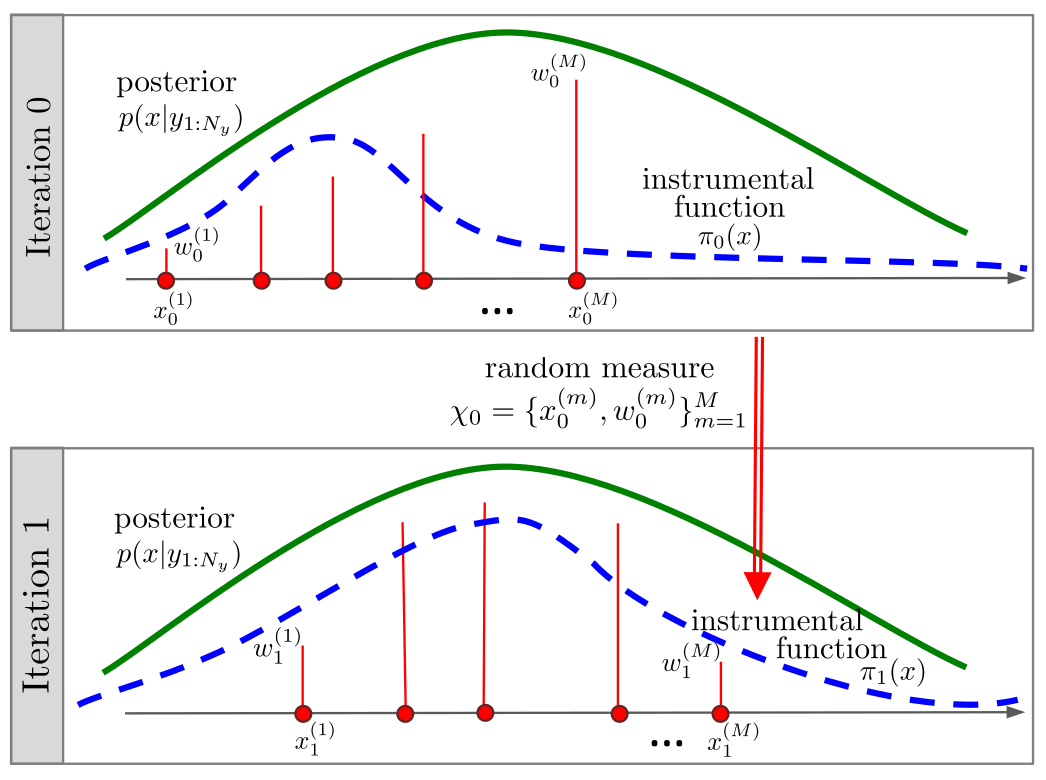
\includegraphics[height=.7\textheight]{\figeco/BMC13-DigitalSignalProc-Fig1}
  $$
  (from \refer{BMC13})
  
}

%====================================================================
\frame{\frametitle{Importance sampling (2/2)} 

  \paragraph{Monte-Carlo E-step.} Importance sampling: 
  \begin{itemize}
    \medskip
    \item For each $1 \leq i \leq n$, sample $\{Z_i^m\}_{1 \leq m \leq M}$ iid $\Ncal(m_i, S_i)$;
    \medskip
    \item Compute the importance weights
    $$
    W_i^m = \frac{p(Z_i^r, Y_i ; x_i)}{\Ncal(Z_i^r; m_i, S_i)}, 
    \qquad
    w_i^m = W_i^m \left/ \left( \sum_{m=1}^M W_i^m \right) \right.;
    $$
    \item Estimate 
    $$
    \widehat{\Esp}( \log p_\theta(Y, Z) \mid Y)
    = \sum_{i=1}^n \sum_{m=1}^M w_i^m \log p_\theta(Z_i^r, Y_i ; x_i).
    $$
  \end{itemize}

  \bigskip \bigskip \pause
  \paragraph{M-step.} Maximize $\widehat{\Esp}( \log p_\theta(Y, Z) \mid Y)$ wrt $\theta$: same problem as VEM.
  
}

%====================================================================
\subsection{Composite likelihood}
%====================================================================
\frame{\frametitle{A reminder on composite likelihood (1/2)} 

  ... but: importance sampling yields poor accuracy even for intermediate dimension $p$.

  \bigskip \bigskip \pause
  \paragraph{Blocks of responses.} Consider $B$ blocks $C_1, \dots C_b$ of responses = subsets of $\{1, \dots p\}$ such that
  \begin{itemize}
    \item all block have same size $k$;
    \item each responses $j$ and each couple of responses $(j, j')$ belongs to at least one block $C_b$.
  \end{itemize}

  \bigskip \bigskip \pause
  \paragraph{Composite likelihood.}
  $$
  \cl(\theta) = \sum_{b=1}^B \lambda_b \log p_\theta(Y^{(b)}; X)
  $$
  where
  \begin{itemize}
    \item $Y^{(b)} =$ responses from block $b$: $\{Y_{ij}\}_{1 \leq i \leq n, j \in C_b}$;
    \item $\lambda_b =$ weight of block $B$ (set to 1).
  \end{itemize}
  
  \bigskip \bigskip \pause
  \paragraph{Example.} $p = 3$, $k = 2$, 
  $$
  \cl(\theta) = \log p_\theta(Y^{1, 2}; X) + \log p_\theta(Y^{1, 3}; X) + \log p_\theta(Y^{2, 3}; X)
  $$
}

%====================================================================
\frame{\frametitle{A reminder on composite likelihood (2/2)}

  \paragraph{Statistical guaranty \refer{VRF11}.} $\widetilde{\theta} = \arg\max_\theta \cl(\theta)$ is
  \begin{itemize}
    \medskip
    \item consistent;
    \medskip
    \item asymptotically normal;
    \medskip
    \item with asymptotic variance matrix = Godambe matrix:
    $$
    \Var_\infty(\widehat{\theta}) = H_\theta J^{-1}_\theta H_\theta
    $$    
    with
    $$
    H_\theta = - \Esp(\nabla^2_\theta \cl(\theta)), 
    \qquad
    J_\theta = \Var(\nabla_\theta \cl(\theta)), 
    $$
  \end{itemize}
  
  \bigskip \bigskip \pause
  \paragraph{MC-EM for Composite likelihood.}
  \begin{itemize}
    \medskip
    \item The decomposition of $\ell(\theta) = \log p_\theta(Y)$ still holds for $\cl(\theta)$;
    \medskip
    \item All quantities (e.g. $\Esp( \log p_\theta(Y^{(b)}, Z^{(b)} \mid Y^{(b)})$ can be estimated by importance sampling.
  \end{itemize}

}

%====================================================================
\subsection{Proposed algorithm}
%====================================================================
\frame{\frametitle{Proposed algorithm}

  \paragraph{Input:} Data $X = n \times d$ and $Y = n \times p$ + Blocks $\{C_b\}_{1 \leq b \leq B}$; 
  
  \bigskip \pause
  \paragraph{Init:} Run VEM to get $\theta^{(0)}$ and $\{(m_i^{(0, b)}$, $S_i^{(0, b)})\}_{1 \leq i \leq n}$;
  
  \bigskip \pause
  \paragraph{Iterate:} at step $h$, for each block $b$, for each $i$:
  \begin{description}
    \pause
    \item[E-step:]
    \begin{enumerate}
      \item Sample $\{Z_i^{h, b, m}\} \sim \Ncal(m_i^{(b, h)}, S_i^{(b, h)})$;
      \item Compute the weigths $w_i^{(h, b, m)}$;
      \item Update $m_i^{(h+1, b)}$ and $S_i^{(h+1, b)}$ according to these weigths;
    \end{enumerate}
    \pause
    \item[M-step:] update 
    $$
    \theta^{(h+1)} = \arg\max_\theta \sum_{i, b, m} \lambda_b w_i^{(h, b, m)} \log p_\theta(Y_i^{(b)}, Z_i^{h, b, m}; x_i);
    $$
  \end{description}
  
  \bigskip \pause
  \paragraph{Stop:} when $\|\theta^{(h+1)} - \theta^{(h)}\| < \varepsilon$;
  
  \bigskip \pause
  \paragraph{Post-process:} use the samples $\{Z_i^{h, b, m}\} \sim \Ncal(m_i^{(b, h)}, S_i^{(b, h)})$ and weigths $w_i^{(h, b, m)}$ to estimate
  $$
  H_\theta, \quad J_\theta \quad \text{and} \quad \Var_\infty(\widehat{\theta}).
  $$

}

%====================================================================
\frame{\frametitle{To do}

  \paragraph{Tuning parameters.}
  \begin{itemize}
    \medskip
    \item Number of particles: actually $M = M^{(h)} \uparrow$ with $h$ (ex.: $M^{(h)} = h M^{(0)}$).
    \medskip
    \item Choosing the blocks: same problems as finding a incomplete (balanced) block design. \\
    \medskip    
    \ra Not that simple for large $p$, but algorithms are available
  \end{itemize}  
  
  \bigskip \bigskip \pause
  \paragraph{Left to do.}
  \begin{itemize}
    \medskip
    \item Finish the code for composite likelihood
    \medskip
    \item Run simulation to assess assymptotic normality
  \end{itemize}

}

%====================================================================
\frame[allowframebreaks]{ \frametitle{References}
  {%\footnotesize
   \footnotesize
   \bibliography{/home/robin/Biblio/BibGene}
%    \bibliographystyle{/home/robin/LATEX/Biblio/astats}
   \bibliographystyle{alpha}
  }
}

%====================================================================
\end{document}
%====================================================================
%====================================================================

  \begin{tabular}{cc}
    \hspace{-.04\textwidth}
    \begin{tabular}{p{.5\textwidth}}
    \end{tabular}
    &
    \begin{tabular}{p{.45\textwidth}}
    \end{tabular}
  \end{tabular}

